\documentclass[a4paper, 12pt]{article}
\usepackage[utf8]{inputenc}
\usepackage[english, ukrainian]{babel}

\usepackage{amsmath, amssymb}
\usepackage{multicol}
\usepackage{graphicx}
\usepackage{float}

\allowdisplaybreaks
\setlength\parindent{0pt}
\numberwithin{equation}{subsection}

\usepackage{hyperref}
\hypersetup{unicode=true,colorlinks=true,linktoc=all,linkcolor=red}

\numberwithin{equation}{subsection}

\renewcommand{\bf}[1]{\textbf{#1}}
\renewcommand{\it}[1]{\textit{#1}}
\newcommand{\bb}[1]{\mathbb{#1}}
\renewcommand{\cal}[1]{\mathcal{#1}}

\renewcommand{\epsilon}{\varepsilon}
\renewcommand{\phi}{\varphi}

\DeclareMathOperator{\diam}{diam}
\DeclareMathOperator{\rang}{rang}
\DeclareMathOperator{\const}{const}

\newenvironment{system}{%
  \begin{equation}%
    \left\{%
      \begin{aligned}%
}{%
      \end{aligned}%
    \right.%
  \end{equation}%
}
\newenvironment{system*}{%
  \begin{equation*}%
    \left\{%
      \begin{aligned}%
}{%
      \end{aligned}%
    \right.%
  \end{equation*}%
}

\makeatletter
\newcommand*{\relrelbarsep}{.386ex}
\newcommand*{\relrelbar}{%
  \mathrel{%
    \mathpalette\@relrelbar\relrelbarsep%
  }%
}
\newcommand*{\@relrelbar}[2]{%
  \raise#2\hbox to 0pt{$\m@th#1\relbar$\hss}%
  \lower#2\hbox{$\m@th#1\relbar$}%
}
\providecommand*{\rightrightarrowsfill@}{%
  \arrowfill@\relrelbar\relrelbar\rightrightarrows%
}
\providecommand*{\leftleftarrowsfill@}{%
  \arrowfill@\leftleftarrows\relrelbar\relrelbar%
}
\providecommand*{\xrightrightarrows}[2][]{%
  \ext@arrow 0359\rightrightarrowsfill@{#1}{#2}%
}
\providecommand*{\xleftleftarrows}[2][]{%
  \ext@arrow 3095\leftleftarrowsfill@{#1}{#2}%
}
\makeatother

\newcommand{\NN}{\mathbb{N}}
\newcommand{\ZZ}{\mathbb{Z}}
\newcommand{\QQ}{\mathbb{Q}}
\newcommand{\RR}{\mathbb{R}}
\newcommand{\CC}{\mathbb{C}}

\newcommand{\Max}{\displaystyle\max\limits}
\newcommand{\Sup}{\displaystyle\sup\limits}
\newcommand{\Sum}{\displaystyle\sum\limits}
\newcommand{\Int}{\displaystyle\int\limits}
\newcommand{\Iint}{\displaystyle\iint\limits}
\newcommand{\Lim}{\displaystyle\lim\limits}

\newcommand*\diff{\mathop{}\!\mathrm{d}}

\newcommand*\rfrac[2]{{}^{#1}\!/_{\!#2}}


\title{{\Huge МАТЕМАТИЧНА ФІЗИКА}}
\author{Скибицький Нікіта}
\date{\today}

\usepackage{amsthm}
\usepackage[dvipsnames]{xcolor}
\usepackage{thmtools}
\usepackage[framemethod=TikZ]{mdframed}

\theoremstyle{definition}
\mdfdefinestyle{mdbluebox}{%
	roundcorner = 10pt,
	linewidth=1pt,
	skipabove=12pt,
	innerbottommargin=9pt,
	skipbelow=2pt,
	nobreak=true,
	linecolor=blue,
	backgroundcolor=TealBlue!5,
}
\declaretheoremstyle[
	headfont=\sffamily\bfseries\color{MidnightBlue},
	mdframed={style=mdbluebox},
	headpunct={\\[3pt]},
	postheadspace={0pt}
]{thmbluebox}

\mdfdefinestyle{mdredbox}{%
	linewidth=0.5pt,
	skipabove=12pt,
	frametitleaboveskip=5pt,
	frametitlebelowskip=0pt,
	skipbelow=2pt,
	frametitlefont=\bfseries,
	innertopmargin=4pt,
	innerbottommargin=8pt,
	nobreak=true,
	linecolor=RawSienna,
	backgroundcolor=Salmon!5,
}
\declaretheoremstyle[
	headfont=\bfseries\color{RawSienna},
	mdframed={style=mdredbox},
	headpunct={\\[3pt]},
	postheadspace={0pt},
]{thmredbox}

\declaretheorem[style=thmbluebox,name=Теорема,numberwithin=subsubsection]{theorem}
\declaretheorem[style=thmbluebox,name=Лема,numberwithin=subsubsection]{lemma}
\declaretheorem[style=thmbluebox,name=Твердження,numberwithin=subsubsection]{proposition}
\declaretheorem[style=thmbluebox,name=Принцип,numberwithin=subsubsection]{th_principle}
\declaretheorem[style=thmbluebox,name=Закон,numberwithin=subsubsection]{law}
\declaretheorem[style=thmbluebox,name=Закон,numbered=no]{law*}
\declaretheorem[style=thmbluebox,name=Формула,numberwithin=subsubsection]{th_formula}
\declaretheorem[style=thmbluebox,name=Рівняння,numberwithin=subsubsection]{th_equation}
\declaretheorem[style=thmbluebox,name=Умова,numberwithin=subsubsection]{th_condition}
\declaretheorem[style=thmbluebox,name=Наслідок,numberwithin=subsubsection]{corollary}

\declaretheorem[style=thmredbox,name=Приклад,numberwithin=subsubsection]{example}
\declaretheorem[style=thmredbox,name=Приклади,sibling=example]{examples}

\declaretheorem[style=thmredbox,name=Властивість,numberwithin=subsubsection]{property}
\declaretheorem[style=thmredbox,name=Властивості,sibling=property]{properties}

\mdfdefinestyle{mdgreenbox}{%
	skipabove=8pt,
	linewidth=2pt,
	rightline=false,
	leftline=true,
	topline=false,
	bottomline=false,
	linecolor=ForestGreen,
	backgroundcolor=ForestGreen!5,
}
\declaretheoremstyle[
	headfont=\bfseries\sffamily\color{ForestGreen!70!black},
	bodyfont=\normalfont,
	spaceabove=2pt,
	spacebelow=1pt,
	mdframed={style=mdgreenbox},
	headpunct={ --- },
]{thmgreenbox}

\mdfdefinestyle{mdblackbox}{%
	skipabove=8pt,
	linewidth=3pt,
	rightline=false,
	leftline=true,
	topline=false,
	bottomline=false,
	linecolor=black,
	backgroundcolor=RedViolet!5!gray!5,
}
\declaretheoremstyle[
	headfont=\bfseries,
	bodyfont=\normalfont\small,
	spaceabove=0pt,
	spacebelow=0pt,
	mdframed={style=mdblackbox}
]{thmblackbox}

\declaretheorem[name=Вправа,numberwithin=subsubsection,style=thmblackbox]{exercise}
\declaretheorem[name=Зауваження,numberwithin=subsubsection,style=thmgreenbox]{remark}
\declaretheorem[name=Визначення,numberwithin=subsubsection,style=thmblackbox]{definition}

\newtheorem{problem}{Задача}[subsection]
\newtheorem{sproblem}[problem]{Задача}
\newtheorem{dproblem}[problem]{Задача}
\renewcommand{\thesproblem}{\theproblem$^{\star}$}
\renewcommand{\thedproblem}{\theproblem$^{\dagger}$}
\newcommand{\listhack}{$\empty$\vspace{-2em}} 

\theoremstyle{remark}
\newtheorem*{solution}{Розв'язок}


\begin{document}

\tableofcontents

\setcounter{section}{3}
\setcounter{subsection}{3}
\setcounter{subsubsection}{9}
\setcounter{theorem}{11}
\setcounter{equation}{50}

\subsubsection{Ізоентропічні течії (течії з постійною ентропією)}

Отримаємо спрощену математичну модель руху ідеальної рідини в припущені, що ентропія ідеальної рідини є величиною постійною в будь-який момент часу і в довільній точці області. \medskip

Виходячи з закону збереження ентропії, за відомою формулою
\begin{equation}
	\nabla \cdot \left( f \vec A \right) = \langle \vec A, \nabla f \rangle + f \left( \nabla \cdot \vec A \right),
\end{equation}
отримаємо:
\begin{equation}
	\rho \cdot \frac{\partial S}{\partial t} + S \cdot \frac{\partial \rho}{\partial t} + \rho \langle V, \nabla S \rangle + S \cdot \big( \nabla \cdot \left( \rho V \right) \big) = 0,
\end{equation}
або враховуючи рівняння нерозривності маємо не дивергентну форму закону збереження ентропії:
\begin{equation}
	\frac{\partial S}{\partial t} + \langle V, \nabla S \rangle = 0.
\end{equation}
	 
Знайдемо повну похідну деякого параметра $f$ вздовж траєкторії руху $x = x(t)$ частинки рідини:
\begin{figure}[H]
	\centering
	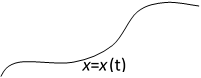
\includegraphics[]{{../img/11-1}.mps}
	\caption{траєкторія руху частинки рідини}
\end{figure}
тобто похідну по часу $t$ вздовж контуру $x = x(t)$:
\begin{equation}
	\frac{\diff f (x(t), t)}{\diff t} = \frac{\partial f}{\partial x_1} \frac{\diff x_1}{\diff t} + \frac{\partial f}{\partial x_2} \frac{\diff x_2}{\diff t} + \frac{\partial f}{\partial x_3} \frac{\diff x_3}{\diff t} + \frac{\partial f}{\partial t} = \frac{\partial f}{\partial t} + \langle V, \nabla f \rangle.
\end{equation}

Будемо називати цей вираз похідною по часу вздовж траєкторії руху частинки. \medskip

З не дивергентної форми закону збереження ентропії бачимо, що повна зміна ентропії вздовж траєкторії руху частинки дорівнює нулю, тобто
\begin{equation}
	\frac{\diff S}{\diff t} = 0.
\end{equation}

Припустимо що в початковий момент часу $t = 0$ ідеальна рідина займає деяку область $\Omega(0)$, а ентропія $S(x, 0) = S_0 = \const$, $\forall x \in \Omega(0)$:
\begin{figure}[H]
	\centering
	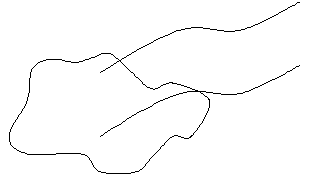
\includegraphics[]{{../img/11-2}.mps}
	\caption{Дві частинки рідини рухаються ``паралельно''}
\end{figure}
 
Тоді згідно $\diff S / \diff t = 0$ в будь-який момент часу $t > 0$ ентропія буде залишатися постійною в довільній точці області, яка утворилася при переміщенні усіх її частинок вздовж траєкторій руху частинок, тобто області $\Omega(t)$. Таким чином можливе існування течій з постійним значення ентропії. Використовуючи введену термодинамічну функцію ентальпію, за формулою
\begin{equation}
	\diff W = T \diff S + \frac{\diff p}{\rho}
\end{equation}
при постійному значенні ентропії $S = \const$ отримаємо співвідношення 
\begin{equation}
	\diff W = \frac{\diff p}{\rho}.	
\end{equation}

Перетворимо закон збереження імпульсу, продиференціюємо відповідні добутки та отримаємо:
\begin{equation}
	V_i  \frac{\partial \rho}{\partial t} + \rho  \frac{\partial V_i}{\partial t} + V_i  \nabla \cdot (\rho V) + \rho \langle V, \nabla V_i \rangle + \nabla_i p = 0.
\end{equation}

Після скорочення отримаємо закон збереження імпульсу в не дивергентній формі:
\begin{equation}
	\frac{\partial V_i}{\partial t} + \langle V, \nabla V_i \rangle + \frac{\nabla_i p}{\rho} = 0.
\end{equation}

Векторна форма якого для ізоентропічних течій має вигляд:
\begin{equation}
	\frac{\partial \vec V}{\partial t} + \langle \vec V, \nabla \vec V \rangle + \nabla W = 0,
\end{equation}
або
\begin{equation}
	\frac{\diff \vec V}{\diff t} + \nabla W = 0
\end{equation}

Скористаємось відомою формулою векторного аналізу
\begin{equation}
	\frac{\nabla |V|^2}{2} = \vec V \times (\nabla \times \vec V) + \langle \vec V, \nabla \vec V \rangle,
\end{equation}
де
\begin{multline}
	\nabla \times \vec V = 
	\begin{vmatrix} 
		i_1 & i_2 & i_3 \\ \\[-.25cm]
		\dfrac{\partial}{\partial x_1} & \dfrac{\partial}{\partial x_2} & \dfrac{\partial}{\partial x_3} \\ \\[-.25cm]
		V_1 & V_2 & V_3
	\end{vmatrix} = \\
	= \vec i_1 \left( \frac{\partial V_3}{\partial x_2} - \frac{\partial V_2}{\partial x_3} \right) - \vec i_2 \left( \frac{\partial V_3}{\partial x_1} - \frac{\partial V_1}{\partial x_3} \right) + \vec i_3 \left( \frac{\partial V_2}{\partial x_1} - \frac{\partial V_1}{\partial x_2} \right).
\end{multline}

Отримаємо рівняння:
\begin{equation}
	\label{eq:3.3.64}
	\frac{\partial V}{\partial t} + \frac{\nabla \left| \vec V\right|^2}{2} - \vec V \times( \nabla \times \vec V) + \nabla W = 0
\end{equation}

Подіємо на нього $\nabla \times$, і врахуємо, що для будь-якої скалярної функції $f$ виуонується $\nabla \times \nabla f = 0$, в результаті отримаємо систему рівнянь відносно вектору швидкості.

\begin{th_equation}[система рівнянь руху ідеальної рідини для ізоентропічного випадку]
	Виконуються співвідношення
	\begin{equation}
		\frac{\partial}{\partial t} \left(\nabla \times \vec V\right) - \nabla \times (\vec V \times (\nabla \times \vec V)) = 0.
	\end{equation}
\end{th_equation}

\subsubsection{Потенціальні течії}

Потенційні течії є частинним випадком ізоентропічних течій. Покажемо можливість існування потенційних течій. \medskip

Розглянемо інтеграл	
\begin{equation}
	\Gamma(t) = \Oint_{c(t)} \vec V(t) \cdot\diff \vec l
\end{equation}
який називається циркуляцією вектора швидкості вздовж контуру (під знаком інтегралу записано скалярний добуток векторів швидкості $\vec V(t)$ та вектору нескінченно малого зміщення вздовж контуру $\diff \vec l$); $c(t)$ --- контур, утворений частинами ідеальної рідини, що рухаються вздовж своїх траєкторій. \medskip

\begin{theorem}[Томсона, про збереження циркуляції векторного поля швидкості]
	Для ізоентропічних течій ($S = \const$) 
	\begin{equation}
	 	\frac{\diff \Gamma}{\diff t} = 0,
	\end{equation}
	тобто циркуляція векторного поля вздовж рухомого рідкого контуру є величина постійна.
\end{theorem}

\begin{proof}
	\begin{align}
		\frac{\diff \Gamma}{\diff t} &= \Oint_{c(t)} \left( \frac{\diff \vec V}{\diff t} \cdot \diff \vec l + \vec V \cdot \diff \frac{\diff \vec l}{\diff t} \right) = \\
		&= \Oint_{c(t)} \left( - \nabla W \cdot \diff l + \vec V \cdot \diff \vec V \right) = \\
		&= \Oint_{c(t)} \diff \left( - W + \frac{|V|^2}{2} \right) = 0.
	\end{align}
\end{proof}

Використаємо теорему Стокса для будь-якої поверхні $\sigma$, що спирається на контур $c(t)$:
\begin{figure}[H]
	\centering
	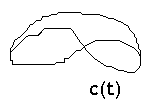
\includegraphics[]{{../img/11-3}.mps}
	\caption{Поверхня $\sigma$ спирається на червоний контур $c(t)$}
\end{figure}

Тобто
\begin{equation}
	\Gamma(t) = \Oint_{c(t)} \vec V(t) \cdot \diff \vec l = \Iint_{\sigma(t)} (\nabla \times V)_n \diff \sigma = \const.
\end{equation}

Розглянемо деяку траєкторію руху $c(t)$ однієї частинки ідеальної рідини і нескінченно малий контур $c_\epsilon(t)$, який нанизаний на траєкторію руху:
\begin{figure}[H]
	\centering
	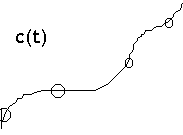
\includegraphics[]{{../img/11-4}.mps}
	\caption{Контур $c_\epsilon(t)$ нанизаний на червону траєкторію $c(t)$}
\end{figure}
 
Припускаючи, що при $t = 0$ маємо $\nabla \times V = 0$, а таким чином $(\nabla \times V)_n = 0$, то згідно теореми Томсона $(\nabla \times V) = 0$, для $t > 0$. \medskip

Якщо розглянути область $\Omega$ для якої циркуляція відсутня при $t = 0$ тобто $\nabla \times V = 0$ то вздовж будь-якої траєкторії яка починається в області $\Omega$ в будь-який момент часу поле залишається безвихровим, тобто $\nabla \times \vec V = 0$:
\begin{figure}[H]
	\centering
	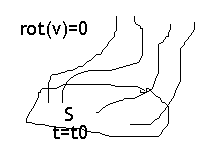
\includegraphics[]{{../img/11-5}.mps}
	\caption{Безвихрове поле: локально рух не паралельний але глобально спрямований паралельно}
\end{figure}

Це свідчить про існування безвихрових або потенційних течій. \medskip

\begin{definition}[потенціальної течії]
	Отже \it{потенціальною} називається течія, для якої
	\begin{equation}
		\forall t \ge t_0, \quad \forall x \in \Omega: \quad \nabla \times \vec V(x, t) = 0.
	\end{equation}
\end{definition}

Звідси випливає, що існує потенціал векторного поля швидкості $\phi$, градієнт якого рівний $\vec V$, тобто $\nabla \phi = \vec V$. Використовуючи формулу \eqref{eq:3.3.64}, де $W$ --- тепловміст, закон збереження імпульсу буде мати вигляд:
\begin{equation}
	\frac{\partial V}{\partial t} = \nabla \left( \frac{|V|^2}{2} + W \right) = 0
\end{equation}

Закон збереження маси запишемо в не дивергентному вигляді
\begin{equation}
	\frac{\partial \rho}{\partial t} + \rho (\nabla \cdot V) + \langle V, \nabla \rho \rangle = 0.
\end{equation}

Проінтегруємо друге рівняння, та врахуємо, що $V = \nabla \phi$, будемо мати:
\begin{equation}
	\nabla \left( \frac{\partial \phi}{\partial t} + \frac{|V|^2}{2} + W \right) = 0
\end{equation}

Звідси  
\begin{equation}
	\frac{\partial \phi}{\partial t} + \frac{|V|^2}{2} + W = \Psi(t), 
\end{equation}
де $\Psi$ --- довільна функція змінної часу. Враховуючи, що потенціал вектору швидкості визначається з точністю до адитивної функції часу, покладемо $\Psi(t) \equiv 0$. Отже, отримали
\begin{th_equation}[інтеграл Коші-Лагранжа]
	Виконуєтсья співвідношення:
	\begin{equation}
		\frac{\partial \phi}{\partial t} + \frac{|V|^2}{2} + W = 0.
	\end{equation}
\end{th_equation}

\begin{definition}[інтеграла Бернуллі]
	Для стаціонарних течій, що не залежать від часу, цей інтеграл називається \it{інтегралом Бернуллі}:
	\begin{equation}
		\frac{|V|^2}{2} + W = \const.
	\end{equation}
\end{definition}

З $\diff W = \diff p / \rho$ випливає, що
\begin{equation}
	\diff W = \frac{1}{\rho} \frac{\diff p}{\diff \rho} \diff p = \frac{1}{\rho} c^2 \diff \rho,
\end{equation}
але $c^2 = \diff p / \diff \rho$, звідки
\begin{equation}
	c^2  \frac{\diff \rho}{\diff t} = \rho  \frac{\diff W}{\diff t}.
\end{equation}

Враховуючи недивергнетну форму рівняння нерозривності отримаємо:
\begin{equation}
	\frac{1}{\rho} \frac{\diff \rho}{\diff t} + \Delta \phi = 0.
\end{equation}

Система рівнянь з інтегралу Коші-Лагранжа та останнього співвідношення є системою двох нелінійних рівнянь з двома змінними і описує потенціальний рух ідеальної рідини. \medskip

З інтегралу Коші-Лагранжа та останнього співвідношення маємо
\begin{equation}
	\frac{1}{c^2} \frac{\diff W}{\diff t} + \Delta \phi = 0.
\end{equation}

Диференціюючи інтеграл Коші-Лагранжа по $t$:
\begin{equation}
	\frac{\diff}{\diff t} \left( \frac{\partial \phi}{\partial t} + \frac{|V|^2}{2} \right) + \frac{\diff W}{\diff t} = 0.
\end{equation}
з урахуванням попереднього рівняння отримаємо:
\begin{equation}
	\frac{\diff}{\diff t} \left( \frac{\partial \phi}{\partial t} + \frac{|\nabla \phi|^2}{2} \right) - c^2 \Delta \phi = 0.
\end{equation}

Це рівняння використовується для дослідження потенціальних течій. Розкриємо це рівняння у тривимірному випадку:
\begin{equation}
	\phi_{tt} + 2 \Sum_{i = 1}^3 V_i \phi_{x_i t} + \Sum_{i,k = 1}^3 V_{x_i} V_{x_k} \phi_{x_i x_k} = c^2 \Sum_{i = 1}^3 \phi_{x_i x_i}.
\end{equation}

Для стаціонарних течій у три- та дво-вимірному випадках маємо:
\begin{multline}
	(c^2 -\phi_x^2)\phi_{xx}+(c^2-\phi_y^2)\phi_{yy}+(c^2-\phi_z^2)\phi_{zz}-\\
	-2(\phi_x\phi_y\phi_{xy}+\phi_z\phi_y\phi_{zy}+\phi_x\phi_z\phi_{xz})=0,
\end{multline}
і
\begin{equation}
	(c^2-\phi_x^2)\phi_{xx}+(c^2-\phi_y^2)\phi_{yy}+2\phi_x\phi_y\phi_{xy}=0.
\end{equation}
відповідно. \medskip

Швидкості звуку у першому з цих рівнянь можна обчислити виходячи з формули Бернулі
\begin{equation}
	W + \frac{|V|^2}{2} = W_0 + \frac{|V_0|^2}{2}.
\end{equation}

Зокрема, для широкого спектру ідеальних газів, з рівнянням стану $\epsilon = p / \rho (\gamma - 1$ можна отримати
\begin{equation}
	c^2 = c_0^2 + \frac{\gamma - 1}{2} \cdot |V_0|^2 - \frac{\gamma - 1}{2} \cdot |V|^2.
\end{equation}

\subsubsection{Модель акустичного руху рідини}

Акустичними рухами ідеальної рідини будемо називати такі її рухи для яких фізичні характеристики рідини мало відрізняються від деяких постійних значень. \medskip

Розглянемо систему
\begin{th_equation}[система рівнянь ізоентропічного руху ідеальної рідини]
	Виконуються співвідношення
	\begin{system}
		& \frac{\partial \rho}{\partial t} + \rho (\nabla \cdot V) + \langle V, \nabla \rho \rangle = 0, \\
		& \frac{\partial V_i}{\partial t} + \langle V, \nabla V_i \rangle + \frac{\nabla_i p}{\rho} = 0, \\
		& S(p, \rho) = S(p_0, \rho_0).
	\end{system}
\end{th_equation}

Відносно параметрів руху будемо припускати, що
\begin{system}
	& p = p_0 + \tilde p, \quad \rho = \rho_0 + \tilde \rho, \quad V = V_0 + \tilde V, \\
	& p_0 = \const, \quad \rho_0 = \const, \quad V_0 = \const = 0, \\
	& \tilde \rho \ll \rho_0, \quad \tilde p \ll p_0, \quad \tilde V \ll 1.
\end{system}

Проведемо лінеаризацію системи рівнянь зберігаючи лише величини першого порядку малості. \medskip

Для першого рівняння системи отримаємо:
\begin{equation}
	\frac{\partial}{\partial t} (\rho_0 + \tilde \rho) + (\rho_0 + \tilde \rho) (\nabla \cdot \tilde V) + \langle \tilde V, \nabla (\rho_0 + \tilde \rho) \rangle = 0.
\end{equation}

Зберігаючи члени першого порядку малості отримаємо
\begin{equation}
	\frac{\partial \tilde \rho}{\partial t} + \rho_0 (\nabla \cdot \tilde V) = 0.
\end{equation}

Для другого рівняння системи маємо
\begin{equation}
	(\rho_0 + \tilde \rho) \left( \frac{\partial \tilde V_i}{\partial t} + \langle \tilde V, \nabla \tilde V_i \rangle \right) + \nabla_i (p_0 + \tilde p) = 0.
\end{equation}

Розкриваючи дужки та нехтуючи членами другого порядку малості отримаємо
\begin{equation}
	\rho_0 \cdot \frac{\partial \tilde V_i}{\partial t} + \nabla_i \tilde p = 0.
\end{equation}

Для лінеаризації третього співвідношення системи, ліву частину співвідношення розкладемо за формулою Тейлора зберігаючи лише члени першого порядку малості
\begin{equation}
	S(p_0 + \tilde p, \rho_0 + \tilde \rho) = S(p_0, \rho_0) + \frac{\partial S(p_0, \rho_0)}{\partial p} \cdot \tilde p + \frac{\partial S(p_0, \rho_0)}{\partial \rho} \cdot \tilde \rho = S(p_0, \rho_0).
\end{equation}

Таким чином можна записати:
\begin{equation}
	\tilde p = - \frac{S_\rho' (p_0, \rho_0)}{S_p'(p_0, \rho_0)} \cdot \tilde \rho,
\end{equation}
або
\begin{equation}
	\tilde p = c_0^2 \tilde \rho.
\end{equation}

Таким чином маємо
\begin{th_equation}[система рівнянь акустики (звукових коливань)]
	Виконуються співвідношення:
	\begin{system}
		& \frac{\partial \tilde \rho}{\partial t} + \rho_0 (\nabla \cdot \tilde V) = 0, \\
		& \rho_0 \cdot \frac{\partial \tilde V_i}{\partial t} + \nabla_i \tilde p = 0, \\
		& \tilde p = c_0^2 \tilde \rho.
	\end{system}
\end{th_equation}

З системи рівнянь можна отримати одне рівняння для тиску, або щільності. \medskip

Для цього перше рівняння продиференціюємо по часу, а на друге векторне рівняння подіємо операцією дивергенція, в результаті будемо мати:
\begin{align}
	\frac{\partial^2 \tilde \rho}{\partial t^2} + \rho_0 \left( \nabla \cdot \frac{\partial \tilde V}{\partial t} \right) &= 0, \\
	\rho_0 \left( \nabla \cdot \frac{\partial \tilde V}{\partial t} \right) + \nabla \cdot \nabla \tilde p &= 0.
\end{align}

Віднімаючи від першого рівняння друге і використовуючи третє рівняння отримаємо
\begin{th_equation}[хвильове]
	Виконується співвідношення:
	\begin{equation}
		\frac{\partial^2 \tilde \rho}{\partial t^2} = c_0^2 \Delta \tilde \rho.
	\end{equation}
\end{th_equation}

Враховуючи потенціальний характер акустичних рухів, вектор швидкості $\tilde V$ можна представити у вигляді градієнту потенціалу і отримати хвильове рівняння відносно потенціалу вектора швидкості.

\subsubsection{Потенційне обтікання тонких тіл}

Розглянемо тонке нерухоме тіло розташоване під малим кутом до плоско паралельного потоку газу, який набігає на це тіло. При певних умовах взаємодії, потік газу навколо тіла можна вважати потенційним, а швидкість газу в околі тіла буде мало відрізняється від вектора швидкості $\vec V_0$ потоку, що набігає з нескінченості. Таким чином вектор швидкості збуреного потоку $\vec V$ можна представити як суму $\vec V = \vec V_0 + \tilde V$. Де $|\tilde V| \ll |\vec V_0|$, тобто збурення внесені тонким тілом є малі по відношенню до набігаючого потоку. \medskip

Виберемо систему координат таким чином, щоби координатна вісь $Ox$ співпадала з напрямом вектора швидкості потоку, що набігає, тобто $\vec V_0 = (\vec V_0^x, 0, 0)$. \medskip

Замість потенціалу $\phi$ повної швидкості $V$ введемо потенціал $\tilde \phi$ швидкості $\tilde V$, тобто $\tilde V = \nabla \tilde \phi$. Зрозуміло, що
\begin{equation}
	\phi = \tilde \phi + x V_0^x.
\end{equation}

Візьмемо за основу нелінійне рівняння для стаціонарної течії у тривимірному просторі і підставимо в нього останнє рівняння, проведемо лінеаризацію рівняння, зберігаючи величини лише першого порядку малості. \medskip

В результаті отримаємо співвідношення
\begin{equation}
	(1 - M_0^2) \cdot \frac{\partial^2 \tilde \phi}{\partial x^2} + \frac{\partial^2 \tilde \phi}{\partial y^2} + \frac{\partial^2 \tilde \phi}{\partial z^2} = 0,
\end{equation}
де $(x, y, z) \in \Omega'$, а $M_0 = V_0^x / c_0$ --- число Маха потоку що набігає.  \medskip

Це рівняння має певну область застосування, зокрема рівняння становиться неприйнятним якщо число $M_0$ близьке до одиниці (біля звукова течія). В цьому випадку коефіцієнт при першому члені є малим, що вимагає збереження членів більш високого порядку малості. На поверхні тіла задається умова непротікання, яку з використанням процесу лінеаризації можна записати у вигляді:
\begin{equation}
	\left( V_0^x + \frac{\partial \tilde \phi}{\partial x} \right) n_x + \frac{\partial \tilde \phi}{\partial y} \cdot n_y  + \frac{\partial \tilde \phi}{\partial z} \cdot n_z  = 0,
\end{equation}
або
\begin{equation}
	\left. \frac{\partial \tilde \phi}{\partial n} \right|_S = -V_0^x n_x.
\end{equation}

В нескінченно віддаленій точці збурений потік співпадає з потоком, що набігає, тому має місце співвідношення:
\begin{equation}
	\tilde \phi \xrightarrow[x, y, z \to \infty]{} 0.
\end{equation}

\end{document}